% Chapter Template

\chapter{Morphing of Local Statistics: Mapping Ensembles through a Resolution Bottleneck} % Main chapter title

Top-Down coarse-grained models aim at reproducing certain experimentally observed phenomenas or to study the consequences upon application of general rules. As such, top-down coarse-grained models are typically not chemically specific. However, in many cases the coarse-grained model incorporates both philosophies, i.e. bottom-up and top-down aspects. Examples of such hybrid models include the Martini forcefield, where a structure-based method is used to tune bonded interactions, and the KG polymer model with a tuned bending potential, which allows to establish a relation to real polymers at the Kuhn scale. While those models can be considered as chemically-specific, they lack the structural fidelity of solely structure-based coarse-grained models. This issue becomes especially apparent when the ensemble of the coarse-grained model is compared with an ensemble of an higher resolution model of the specific system mapped to the coarse-grained resolution. 

In this chapter, a method to improve the quality of molecular structures obtained with hybrid top-down models is investigated. In particular, the method aims at morphing local statistics in order to resemble a given target distribution more closely. To this end, a local scale is introduced that defines the extent to which features are allowed to change. Specifically, molecular structures of an initial distribution are further coarse-grained up to this scale. Afterwards, DBM is applied to reintroduce local features learned from examples of the target system. 

The motivation for this project is to introduce a two-step backmapping scheme for hybrid top-down coarse-grained models. Backmapping of imperfect molecular structures is expected to yield unphysical artifacts. In order to reduce such artifacts already on the coarse-grained scale, local statistics of the coarse-grained structure are corrected before serving it as an input for the backmapping algorithm. 

In the following, the method is applied to two systems: (1) A condensed-phase system of the alkene tetracosane sampled with the Martini forcefield and (2) a polymer melt of sPS sampled with the KG moldel with additional bending potential. The content presented in this chapter is not published yet.

\label{morphing} % Change X to a consecutive number; for referencing this chapter elsewhere, use \ref{ChapterX}

\begin{figure}
  \centering
      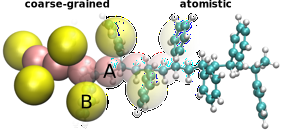
\includegraphics[width=1.0\textwidth]{./Figures/morphing/intro.png}
  \caption{morphbm}
  \label{FIG:TET_morphbm}
\end{figure}


\section{Method}

The method applied in this chapter aims at morphing local features of molecular structures by passing them through a resolution bottleneck. The idea is inspired by the concept of cross-modal learning (CML) known in the ML community.\cite{feng2014cross, cao2016correlation, mukherjee2017deep, yoo2019image} CML is used to link sources of information from different domains, such as audio-to-image translation. In its core, two autoencoder $A$ and $B$ are trained to encode and decode samples $\mathbf{a}$ and $\mathbf{b}$ from two different distributions $\mathcal{A}$ and $\mathcal{B}$. Cross-connecting the encoder $e$ and decoder $d$ of both models, i.e. $d_B\big(e_A(\mathbf{a})\big)$ and $d_A\big(e_B(\mathbf{b})\big)$ respectively, aims at mapping between the distributions $\mathcal{A}$ and $\mathcal{B}$. However, connecting the latent distribtions of both models, i.e. the information-bottleneck, is challenging and subject to current research.\cite{wang2016comprehensive}

Here, two distributions of molecular structures $\mathcal{X}$ and $\mathcal{Y}$ are given, where the resolution of both distributions is equivalent. While the ultimate goal is to introduce a ML based mapping function $g_{\Theta}$ from one distribution to the other, i.e. $g_{\Theta}(\mathcal{X}) \approx \mathcal{Y}$, it is investigated if such a mapping can be realized by changing features only on a local scale. In other words, it is hypothesized that both distributions match at a lower resolution. To this end, a simple encoder $e_s$, i.e. a fine-to-coarse mapping of the coordinates, is chosen that reduces the number of particles $n$ by a factor $s$

\begin{equation}
 e_{s}: \mathbb{R}^{3n} \rightarrow \mathbb{R}^{3n/s} .
\end{equation}

Specifically, $e_n$ computes the center of mass for groups of $n$ particles. Afterwards, the coarse-grained structure is backmapped utilizing DBM as explained in Sec. \ref{methology}. Importantly, DBM is trained solely on structures drawn from the target distribution $\mathcal{Y}$ but deployed for coarse-grained structures drawn from the input distribution $\mathcal{X}$. As such, local features removed by $e_s$ are reinserted based on the local correlations learned from $\mathcal{Y}$. 

Deploying different values for the coarse-graining factor $s$ allows to scale the extent to which local features are allowed to change. Assuming that the backmapping scheme yields a perfect reconstruction, the mapping $g_{\Theta}(e_s(\mathcal{X}))$ is expected to yield a more accurate reproduction of $\mathcal{Y}$ the larger $s$ becomes, since the reinsertion of details becomes less restricted by the coarse-grained representation. However, larger values of $s$ lead to a more complex backmapping excercise. As such, chosing the value for $s$ is a trade-off between the complexity of the backmapping task and the impact of the morphing. 

The proposed method is solely data driven, i.e it avoids to parametrize a forcefield for the given target distribution. However, the quality of morphed structures can be improved by incorporating an artificial energy landscape that penalizes forbitten configurations in terms of bond lengths, angles and non-bonded distances. In particular, a harmonic potential of the form

\begin{equation}
 U(s) =
  \begin{cases}
      a(s - s_{\text{min}})^2,& s < s_{\text{min}}\\
      a(s - s_{\text{max}})^2,& s > s_{\text{max}}\\
      0,              & \text{otherwise},
  \end{cases}
\end{equation}

is applied as bonded interaction, where $s$ represents bond lengths and angles, respectively, and $a$ is a scaling factor.  Similarly, a harmonic potential for non-bonded distances $d$

\begin{equation}
 U(d) =
  \begin{cases}
      a(1 - \frac{d}{d_{\text{min}}})^2,& d < d_{\text{min}}\\
      0,              & \text{otherwise},
  \end{cases}
\end{equation}

is introduced, where $d_{\text{min}}$ is the minimum distance for non-bonded particles. The values for the minimum and maximum distances/angles are obtained from distributions of the target system.


\section{Martini Model: Tetracosane}

\begin{figure}
  \centering
      \includegraphics[width=0.8\textwidth]{./Figures/morphing/tetracosane/morphbm_ff_dists.pdf}
  \caption{morphbm}
  \label{FIG:TET_morphbm}
\end{figure}

\begin{figure}
  \centering
      \includegraphics[width=0.8\textwidth]{./Figures/morphing/tetracosane/morphgibbs_ff_dists.pdf}
  \caption{morphgibbs}
  \label{FIG:TET_morphgibbs}
\end{figure}

\begin{figure}
  \centering
      \includegraphics[width=1.1\textwidth]{./Figures/morphing/tetracosane/free_energy.pdf}
  \caption{SM free energy}
  \label{FIG:TET_morphgibbs}
\end{figure}

\section{Kremer-Grest Model: Synditactic Polystyrene}

\begin{figure}
  \centering
      \includegraphics[width=0.8\textwidth]{./Figures/morphing/sPS/morph_ff_dists.pdf}
  \caption{morphgibbs}
  \label{FIG:TET_morphgibbs}
\end{figure}

\begin{figure}
  \centering
      \includegraphics[width=1.1\textwidth]{./Figures/morphing/sPS/free_energy.pdf}
  \caption{SM free energy}
  \label{FIG:TET_morphgibbs}
\end{figure}

\section{Discussion}
